% arara: pdflatex: { synctex: yes, shell: yes }

% A primeira linha do ficheiro indica ao programa 'arara' como compilar
% o documento. Existem várias maneiras diferentes de compilar, mas esta
% primeira linha pode em geral ser ignorada.

% Este comando, o primeiro do documento, importa a classe a usar. Cada
% documento só pode ter uma classe.
\documentclass[portuguese]{ist-thesis}

% Entre 'documentclass' e 'begin{document}' encontra-se o 'preamble', ou
% a secção de código para importar packages e estabelecer configurações
% para o documento todo. A classe importa algumas packages básicas por
% defeito, mas aqui estão outras packages também úteis para uma tese.
% Qualquer package pode ser importada, que em geral não gera conflito.
% Recomendo consultar a documentação de cada package no site 'ctan.org'.

% Configurações para citações internacionais
\usepackage{csquotes}

% Gestão de bibliografia e citações
\usepackage{biblatex}
\addbibresource{main.bib}

% Introdução de texto de exemplo
\usepackage{lipsum}

% Estilo diferente de tabelas
\usepackage{booktabs}

% Packages para esboçar gráficos e diagramas
\usepackage{tikz}
\usepackage{pgfplots}
\usetikzlibrary{positioning,arrows.meta}

% Alterar as pastas de onde importar imagens (/graphics/) e dados de
% vários tipos (/data/)
\graphicspath{{graphics/}}
\pgfplotsset{table/search path = {data}}

% Comando próprio da classe
% Define a imagem de capa pelo nome, com o tamanho entre parênteses
% retos (fracção da largura da página, neste caso metade)
\setcoverimage[0.5]{example-image-a}

% Fim do 'preamble' e início do documento escrito
\begin{document}

% Comando próprio da classe
% Cria a capa com base nos dados fornecidos no 'preamble' com comandos
% próprios
\makecover

% Ambiente próprio da classe
% Formata o texto no seu interior como dedicatória
\begin{dedication}
	\lipsum[1] % Introduz um parágrafo de 'lorem ipsum', ou texto exemplo
\end{dedication}

% Ambiente próprio da classe
% Formata o texto no seu interior como agradecimentos
\begin{acknowledgements}
	\lipsum[2] % Introduz um parágrafo de 'lorem ipsum', ou texto exemplo
\end{acknowledgements}

% Ambiente próprio da classe
% Formata o texto no seu interior como resumo, aceitando palavras-chave
% como um argumento extra
\begin{tabstract}{Resumo, Palavras-Chave, Resumo Analítico, \textit{Abstract}}
	Resumo e palavras-chave (em português e em inglês). O resumo analítico, também designado por resumo ou abstract, descreve o objectivo, o conteúdo do trabalho e as conclusões. Deve ser escrito em português e inglês, com um máximo de 250 palavras cada e acompanhado de 4 a 6 palavras-chave.
	The abstract describes the objective, the content of the project and the conclusions. It must be written in both portuguese and english, with a maximum of 250 words, accompanied by 4 to 6 keywords.
\end{tabstract}

% Índice
\tableofcontents

% Lista de figuras
\listoffigures

% Lista de tabelas
\listoftables

% Comando próprio da classe
% Finaliza a parte inicial do documento, e começa o texto escrito
% propriamente dito. Utilizado pela classe para definir coisas como
% o tipo de numeração
\mainstart

\chapter{Introdução}

\lipsum[1] % Introduz um parágrafo de 'lorem ipsum', ou texto exemplo

\section{Primeira Secção}

Esta referência liga à equação \eqref{eq:equation1}.

\begin{gather}\label{eq:equation1}
	\mathbb{P}\left(\frac{X_1 + \cdots + X_n}{\sqrt{n}} \leq y\right) \rightarrow \mathrm{R}(y) = \int_{-\infty}^{y} \frac{e^{-t^2/2}}{\sqrt{2\pi}}dt \qquad \mathrm{as} \quad n \rightarrow \infty
\end{gather}

\lipsum[2-3] % Introduz um parágrafo de 'lorem ipsum', ou texto exemplo

\begin{figure}[ht]
	\centering
	\includegraphics[width = 0.5\linewidth]{example-image}
	\caption{Imagem de exemplo.}
	\label{fig:image1}
\end{figure}

\lipsum[1] % Introduz um parágrafo de 'lorem ipsum', ou texto exemplo

\begin{table}[ht]
	\centering
	\caption{Algumas expressões e variáveis. Nas tabelas, a legenda vem em cima.}
	\begin{tabular}{c c c}\toprule
		\textbf{Expression}	& \textbf{Value of $\mathbf{x}$}	& \textbf{Value of $\mathbf{y}$}\\
		\midrule
		$y = 4x$			& $67$								& $268$							\\
		$y = x^2$			& $13$								& $169$							\\
		$y = e^x$			& $9.5$								& $33.115$						\\
		\bottomrule
	\end{tabular}
	\label{tab:tab1}
\end{table}

\lipsum[11] % Introduz um parágrafo de 'lorem ipsum', ou texto exemplo

\begin{figure}[ht]
	\centering
	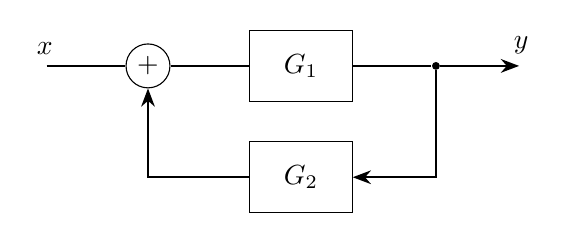
\begin{tikzpicture}
		\tikzstyle{mainblock} = [rectangle, draw, align = center, minimum height = 9mm, minimum width = 13mm];
		\tikzstyle{sum} = [circle, draw, align = center, inner sep = 2pt];
		\tikzstyle{mainpath} = [draw, thick, -{Stealth[]}];
		\node (start) at (0,0) [inner sep = 0mm, label = {90:$x$}] {};
		\node (sum1) [sum, right=of start] {$+$};
		\node (g1) [mainblock, right=of sum1] {$G_1$};
		\node (ex1) [circle, fill, inner sep = 1pt, right=of g1] {};
		\node (end) [right=of ex1, inner sep = 0mm, label = {90:$y$}] {};
		\node (g2) [mainblock, below=5mm of g1] {$G_2$};
		\path [mainpath] (start) -- (sum1) -- (g1) -- (ex1) -- (end);
		\path (ex1) -- (ex1 |- g2) [mainpath] --  (g2);
		\path (g2) -- (g2 -| sum1) [mainpath] -- (sum1);
	\end{tikzpicture}
	\caption{Exemplo de um diagrama feito em \LaTeX{}.}
	\label{fig:diag1}
\end{figure}

\lipsum[13-14] % Introduz um parágrafo de 'lorem ipsum', ou texto exemplo

\begin{figure}
	\centering
	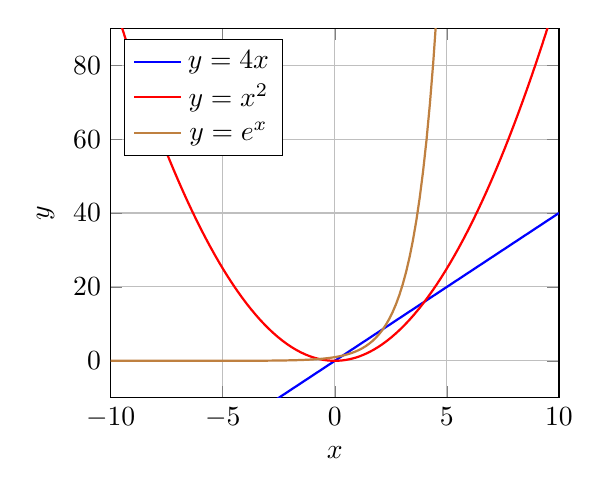
\begin{tikzpicture}
		\begin{axis}
				[width = 0.6\linewidth,
				samples = 100,
				grid = both,
				xmin = -10, xmax = 10,
				ymin = -10, ymax = 90,
				xlabel = {$x$},
				ylabel = {$y$},
				legend pos = north west,]
			\addplot [mark = none, color = blue, thick, domain = -10:10] {4*x};
			\addplot [mark = none, color = red, thick, domain = -10:10] {x^2};
			\addplot [mark = none, color = brown, thick, domain = -10:5] {e^x};
			\legend{$y = 4x$,$y = x^2$,$y = e^x$};
		\end{axis}
	\end{tikzpicture}
	\caption{Exemplo de um gráfico em \LaTeX{}.}
	\label{fig:graph1}
\end{figure}

\lipsum[15] % Introduz um parágrafo de 'lorem ipsum', ou texto exemplo

\begin{figure}
	\centering
	\begin{tikzpicture}
		\begin{axis}
				[width = 0.9\linewidth,
				height = 0.6\linewidth,
				xmin = 5,
				grid = both,
				xlabel = {Tempo ($x$)},
				ylabel = {Amplitude},
				legend pos = north east,]
			\addplot [red] table [col sep = comma, x index = 0, y index = 1, mark = none] {data_example.csv};
			\legend{Exemplo};
		\end{axis}
	\end{tikzpicture}
	\caption[Exemplo de um \textit{plot} de dados em \LaTeX{}.]{Exemplo de um \textit{plot} de dados em \LaTeX{}. Os dados foram obtidos de um ficheiro \texttt{.csv} auxiliar.}
	\label{fig:graph1}
\end{figure}

\lipsum % Introduz um parágrafo de 'lorem ipsum', ou texto exemplo

% Citações vazias. Permite à bibliografia incluir as referências sem
% citações no texto.
\nocite{latex-companion, fontcatalogue, latexwiki, ctan, texsx}

% Introduz a bibliografia. A opção 'heading = bibintoc' introduz a
% bibliografia no índice.
\printbibliography[heading = bibintoc]

\end{document}
